\documentclass[10pt,a4paper]{article}
\usepackage[latin1]{inputenc}
\usepackage{amsmath}
\usepackage{amsfonts}
\usepackage{amssymb}
\usepackage{graphicx}

\begin{document}
\section{ASSIGNMENT NO: A6}
Author:\:   Ameeth Kanawaday\\
Roll No:\:  4430\\
\section{Problem Definition}
Implement a simple approach for k-means/ k-medoids clustering using C++.

\section{Learning Objectives:}
\begin{enumerate}
\item To understand the concept of clustering.
\item To implement k-means clustering algorithm.
\end{enumerate}

\section{S/W and H/W requirements:}
\begin{enumerate}
\item Open source 64 bit OS.
\item Gedit text editor.
\item C++ programming language.
\item g++ compiler.
\end{enumerate}

\section{Theory}
\textbf{k-means Clustering:}
\\\\
k-means clustering is a method of vector quantization, originally from signal processing, that is popular for cluster analysis in data mining. k-means clustering aims to partition n observations into k clusters in which each observation belongs to the cluster with the nearest mean, serving as a prototype of the cluster. This results in a partitioning of the data space into Voronoi cells.
\\\\
The problem is computationally difficult (NP-hard); however, there are efficient heuristic algorithms that are commonly employed and converge quickly to a local optimum. These are usually similar to the expectation-maximization algorithm for mixtures of Gaussian distributions via an iterative refinement approach employed by both algorithms. Additionally, they both use cluster centers to model the data; however, k-means clustering tends to find clusters of comparable spatial extent, while the expectation-maximization mechanism allows clusters to have different shapes.
\\\\
The algorithm has a loose relationship to the k-nearest neighbor classifier, a popular machine learning technique for classification that is often confused with k-means because of the k in the name. One can apply the 1-nearest neighbor classifier on the cluster centers obtained by k-means to classify new data into the existing clusters. This is known as nearest centroid classifier or Rocchio algorithm.
\\\\
\\\\
Given a set of observations (x1, x2,..., xn), where each observation is a d-dimensional real vector, k-means clustering aims to partition the n observations into k (<= n) sets S = {S1, S2,..., Sk} so as to minimize the within-cluster sum of squares (WCSS) (sum of distance functions of each point in the cluster to the K center). In other words, its objective is to find:
\\\\
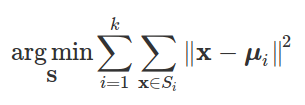
\includegraphics[scale=0.5]{im1.png}
\\\\
\textbf{Algorithm:}
\\\\
Let  X = {x1,x2,x3,...,xn} be the set of data points and V = {v1,v2...,vc} be the set of centers.
\begin{enumerate}
\item Randomly select 'c' cluster centers.
\item Calculate the distance between each data point and cluster centers.
\item Assign the data point to the cluster center whose distance from the cluster center is minimum of all the cluster centers.
\item Recalculate the new cluster center using:
\\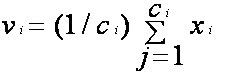
\includegraphics[scale=0.5]{im2.png}
\\\\where, 'ci' represents the number of data points in ith cluster.
\item Recalculate the distance between each data point and new obtained cluster centers.
\item If no data point was reassigned then stop, otherwise repeat from step 3).
\end{enumerate}

\section{Related Mathematics}
Let S be the solution perspective of the given problem.
\\The set S is defined as:
\\$S=\lbrace\ s,e,X,Y,F,DD,NDD|\varnothing_{s}\rbrace$
\\Where,
\\s= Start point 
\\s= data set of points i.e. {x1,x2,...,xn}
\\e= End point 
\\e= k clusters {C1,C2,...,Ck}, such that,
\\$C1 U C2 U...U Ck = {x1,x2,...,xn}$, and
\\$C1 \cap C2 \cap ... \cap Ck = \phi$
\\F= Set of main functions
\\DD= set of deterministic data
\\NDD= set of non deterministic data
\\\\X= Input Set.
\\$X=\lbrace\ x_{1},x_{2},...,x_{n},k \rbrace$
\\where,
\\$x_{i}$= data points
\\k= no. of clusters
\\\\ Y = $\lbrace C1, C2, ..., Ck \rbrace$
\\where, Ci = ith cluster.
\\\\ F = $\lbrace f_{choose}, f_{dist}, f_{avg}, f_{assign} \rbrace$
\\\\$f_{choose}$  :function to choose random centroids.
\\\\ $f_{dist}$ :function to calculate distance of data points from the centroids.
\\\\ $f_{average}$ :function to calculate average of all the points in a cluster and update the centroid of that cluster.
\\\\ $f_{ack}$ :function to assign a data point to the nearest cluster.
\\\\ DD = $\lbrace x_{1},x_{2},...,x_{n},k \rbrace$
\\ NDD = $\lbrace initial centroids \rbrace$


\section{State Diagram}
\includegraphics[scale=0.5]{cl1a6.png}
\\q0 = select random centroids
\\q1 = assign points to clusters
\\q2 = cluster centroid update state
\\q3 = display final clusters state
\\qf = final state

\section{Program}
\begin{verbatim}
 PROGRAM

filename: a6.cpp

#include<iostream>
#include<stdio.h>
#include<time.h>
#include<stdlib.h>
using namespace std;

class kmeans
{

struct points
{
 float x;
 float y;
};
public:
struct points p[8];
struct points c[3];
void input();
int km();
float distance(float a,float b,float x,float y);
};
int tally[8][10];
int count;
int n;

void kmeans::input()
{
 p[0].x=2;p[0].y=2;
 p[1].x=1;p[1].y=14;
 p[2].x=10;p[2].y=7;
 p[3].x=1;p[3].y=11;
 p[4].x=3;p[4].y=4;
 p[5].x=11;p[5].y=8;
 p[6].x=4;p[6].y=3;
 p[7].x=12;p[7].y=2;
int i,random=0;
srand(time(NULL));
for(i=0;i<3;i++)
{
 random=(rand())%7;
 c[i].x=p[random].x;
 c[i].y=p[random].y;
}
}

float kmeans::distance(float a,float b,float x,float y)
{
float t1=a-x;
float t2=b-y;
if(t1<0)
 t1=-t1;
if(t2<0)
 t2=-t2;
return (t1+t2);
}

int kmeans::km()
{
int i,j;
float table[8][4];
for(i=0;i<n;i++)
{
 table[i][0]=distance(p[i].x,p[i].y,c[0].x,c[0].y);
 table[i][1]=distance(p[i].x,p[i].y,c[1].x,c[1].y);
 table[i][2]=distance(p[i].x,p[i].y,c[2].x,c[2].y);
 if(table[i][0]<=table[i][1] && table[i][0]<=table[i][2])
 {
  tally[i][count]=0;
  table[i][3]=table[i][0];
 }
 else if(table[i][1]<=table[i][0] && table[i][1]<=table[i][2])
 {
  tally[i][count]=1;
  table[i][3]=table[i][1];
 }
 else if(table[i][2]<=table[i][0] && table[i][2]<=table[i][1])
 {
  tally[i][count]=2;
  table[i][3]=table[i][2];
 }
}
cout<<"TABLE: "<<count+1<<endl;
cout<<"Centroids are: ("<<c[0].x<<","<<c[0].y<<"), 
("<<c[1].x<<","<<c[1].y<<"), ("<<c[2].x<<","<<c[2].y<<")"<<endl;

cout<<"c1\tc2\tc3\tmin"<<endl;
cout<<"-------------------------"<<endl;
for(i=0;i<n;i++)
{
 for(j=0;j<4;j++)
 {
 cout<<table[i][j]<<"\t";
 }
cout<<endl;
}
cout<<"-------------------------"<<endl;

float c0=0,c1=0,c2=0,c0x=0,c0y=0,c1x=0,c1y=0,c2x=0,c2y=0;
for(i=0;i<n;i++)
{
if(tally[i][count]==0)
{
c0x+=p[i].x;
c0y+=p[i].y;
c0++;
}
else if(tally[i][count]==1)
{
c1x+=p[i].x;
c1y+=p[i].y;
c1++;
}
else if(tally[i][count]==2)
{
c2x+=p[i].x;
c2y+=p[i].y;
c2++;
}
}
c[0].x=c0x/c0;
c[0].y=c0y/c0;
c[1].x=c1x/c1;
c[1].y=c1y/c1;
c[2].x=c2x/c2;
c[2].y=c2y/c2;

int flag=0;
if(count!=0)
{
for(i=0;i<n;i++)
{
 if(tally[i][count]==tally[i][count-1])
   flag++;
}
}
count++;
return flag;
}

int main()
{
kmeans k;
k.input();
n=8;
count=0;
int flag=k.km();
while(flag!=8)
 flag=k.km();
if(flag==8)
 cout<<"Centroids found"<<endl;
for(int i=0;i<n;i++)
{
 for(int j=0;j<count;j++)
  cout<<tally[i][j]<<"  ";
 cout<<endl;
}
return 0;
}


OUTPUT

ameeth@ubuntu-16.0.4:~/CL1$ ./a.out
TABLE: 1
Centroids are: (3,4), (1,14), (2,2)
c1	c2	c3	min
-------------------------
3	13	0	0	
12	0	13	0	
10	16	13	10	
9	3	10	3	
0	12	3	0	
12	16	15	12	
2	14	3	2	
11	23	10	10	
-------------------------
TABLE: 2
Centroids are: (7,5.5), (1,12.5), (7,2)
c1	c2	c3	min
-------------------------
8.5	11.5	5	5	
14.5	1.5	18	1.5	
4.5	14.5	8	4.5	
11.5	1.5	15	1.5	
5.5	10.5	6	5.5	
6.5	14.5	10	6.5	
5.5	12.5	4	4	
8.5	21.5	5	5	
-------------------------
TABLE: 3
Centroids are: (8,6.33333), (1,12.5), (6,2.33333)
c1	c2	c3	min
-------------------------
10.3333	11.5	4.33333	4.33333	
14.6667	1.5	16.6667	1.5	
2.66667	14.5	8.66667	2.66667	
11.6667	1.5	13.6667	1.5	
7.33333	10.5	4.66667	4.66667	
4.66667	14.5	10.6667	4.66667	
7.33333	12.5	2.66667	2.66667	
8.33333	21.5	6.33333	6.33333	
-------------------------
TABLE: 4
Centroids are: (10.5,7.5), (1,12.5), (5.25,2.75)
c1	c2	c3	min
-------------------------
14	11.5	4	4	
16	1.5	15.5	1.5	
1	14.5	9	1	
13	1.5	12.5	1.5	
11	10.5	3.5	3.5	
1	14.5	11	1	
11	12.5	1.5	1.5	
7	21.5	7.5	7	
-------------------------
TABLE: 5
Centroids are: (11,5.66667), (1,12.5), (3,3)
c1	c2	c3	min
-------------------------
12.6667	11.5	2	2	
18.3333	1.5	13	1.5	
2.33333	14.5	11	2.33333	
15.3333	1.5	10	1.5	
9.66667	10.5	1	1	
2.33333	14.5	13	2.33333	
9.66667	12.5	1	1	
4.66667	21.5	10	4.66667	
-------------------------
Centroids found
2  2  2  2  2  
1  1  1  1  1  
0  0  0  0  0  
1  1  1  1  1  
0  0  2  2  2  
0  0  0  0  0  
0  2  2  2  2  
2  2  2  0  0  
ameeth@ubuntu-16.0.4:~/CL1$ 




\end{verbatim}
\section{Conclusion}
Thus we have implemented the Naive Bayes classifier in python using sklearn.
\end{document}